\documentclass{jhwhw}
\usepackage{amsmath}
\usepackage{amssymb}
\usepackage{tikz}
\title{MATH 5510: Topology: HW 1}
\author{Markus Foote}

\begin{document}
\problem{}%1
    Let $$d_{(2)}(x,y)=\sqrt{(x_1-y_1)^2+\cdots+(x_n-y_n)^2}$$ be the Euclidean distance function in $\mathbb{R}^n$ and let $$d_{(1)}(x,y)=|x_1-y_1|+\cdots+|x_n-y_n|$$ be the ''taxicab'' distance, where, as usual, $x=(x_1,\dots,x_n)$ and$y=(y_1,\dots,y_n)$. Prove the following two inequalities that compare the two distances and discuss the case of equality in each inequality. $$d_{(2)}(x,y)\leq d_{(1)}(x,y)\leq \sqrt{n}\,d_{(2)}(x,y).$$
\solution
\part
Prove $d_{(2)}(x,y)\leq d_{(1)}(x,y)$.
\begin{align}
d_{(2)}(x,y)&\leq d_{(1)}(x,y)\\
(d_{(2)}(x,y))^2&\leq (d_{(1)}(x,y))^2\\
\big(\sqrt{(x_1-y_1)^2+\cdots+(x_n-y_n)^2}\big)^2&\leq \big(|x_1-y_1|+\cdots+|x_n-y_n|\big)^2\\
(x_1-y_1)^2+\cdots+(x_n-y_n)^2 &\leq \big(|x_1-y_1|+\cdots+|x_n-y_n|\big)^2\\
\sum_{i=1}^{n}\left[(x_i-y_i)^2\right] &\leq \left(\sum_{i=1}^{n}|x_i-y_i|\right)^2\\
\sum_{i=1}^{n}\left[(x_i-y_i)^2\right] &\leq \left(\sum_{i=1}^{n}|x_i-y_i|\right)\left(\sum_{j=1}^{n}|x_j-y_j|\right)\\
\sum_{i=1}^{n}\left[(x_i-y_i)^2\right] &\leq \sum_{i=1}^{n}\left[|x_i-y_i|\left(|x_i-y_i|+\sum_{j=1,\,j\neq i}^{n}|x_j-y_j|\right)\right]\\
\sum_{i=1}^{n}\left[(x_i-y_i)^2\right] &\leq \sum_{i=1}^{n}|x_i-y_i|^2+\sum_{j=1,\,j\neq i}^{n}|x_i-y_i||x_j-y_j|\\
\sum_{i=1}^{n}\left[(x_i-y_i)^2\right] &\leq \sum_{i=1}^{n}\left(x_i-y_i\right)^2+\sum_{i=1}^{n}\sum_{j=1,\,j\neq i}^{n}|x_i-y_i||x_j-y_j|\\
0 &\leq \sum_{i=1}^{n}\sum_{j=1,\,j\neq i}^{n}|x_i-y_i||x_j-y_j|
\end{align}
The trivial case of equality is both points being zero. More interestingly, points that differ in only one dimension and are equal in all other dimensions have the same distance in both metrics.
\part
$d_{(1)(x,y)} \le \sqrt{n}\,d_{(2)}(x,y)$
\begin{align}
d_{(1)}(x,y)&=\sum_{i=1}^{n}|x_i-y_i|\\
             &=\sum_{i=1}^{n}\Big(|x_i-y_i| \cdot 1\Big)                 \\
             & \left(\sum_{i=1}^{n}\Big(|x_i-y_i| \cdot 1\Big)\right)^2 &\le& \left(\sum_{i=1}^{n}|x_i-y_i|^2\right)\left(\sum_{i=1}^{n} 1^2 \right)\\
             &= \sum_{i=1}^{n}\Big(|x_i-y_i| \cdot 1\Big)                  &\le& \left(\sum_{i=1}^{n}|x_i-y_i|^2\right)^{\frac{1}{2}}\left(\sum_{i=1}^{n} 1^2 \right)^{\frac{1}{2}}\\
             &                                                                               &\le& \sqrt{n}\left(\sum_{i=1}^{n}|x_i-y_i|^2\right)^{\frac{1}{2}} &= \sqrt{n}\,d_{(2)}(x,y)
\end{align}
Equality occurs trivially when both points are zero. More interestingly, equality occurs when the points are equally distant on the real line for each dimension, which might be visualized as the two points being the opposite corners of a square, cube, hypercube, etc. The metrics are also always equal for $\mathbb{R}^1$.

\problem{}%2
Let $f:[0,\infty)\to [0,\infty)$ be a function that satisfies: 
\begin{enumerate}
	\item $f(0) = 0$.
	\item $f$ is strictly increasing: $f(s) < f(t) $ whenever $0\le s < t $.
	\item $f(s+t)\le f(s) + f(t)$ for all $s,t\ge 0$.
\end{enumerate}
Prove that If $(X,d)$ is a metric space, $(X,f\circ d)$ is also a metric space.
\solution
We must prove the axioms of a metric space with the new metric $f\circ d$:
\begin{enumerate}
	\item $f\circ d(x,y) \geq 0$, $f\circ d(x,y) =0$ if and only if $x=y$. 
	
	$d$ is a metric, thus $d=0$ if and only if $x=y$. Given that $f(0)=0$ we know that $f\circ d=0$ when $d=0$. Furthermore, because $f$ is strictly increasing, we know that this is the only argument that will produce zero. Also, $f\circ d$ is strictly increasing from zero, thus $f\circ d(x,y) \ge 0$, thus the axiom holds.
	\item $f\circ d(x,y)=f\circ d(y,x)$
	
	$d$ is a metric, thus $d(x,y)=d(y,x)$. As $f$ is a function, the same input argument will always produce the same output value, thus the axiom holds.
	\item $f\circ d(x,z) \leq f\circ d(x,y) + f\circ d(y,z)$
	
	Let $d(x,y)=s$ and $d(y,z)=t$, thus $d(x,z) \le s+t$ as $d$ is a metric. As $f$ is strictly increasing, $f\circ d(x,z) \le f(s+t)$. Furthermore, it is given that $f(s+t)\le f(s) + f(t)$, thus $f\circ d(x,z) \le f(s) + f(t)$, which is $f\circ d(x,z) \le f\circ d(x,y) + f\circ d(y,z)$ which is the triangle inequality.
\end{enumerate}
\problem{}%3
Which of the following functions $d:\mathbb{R}\times \mathbb{R} \to \mathbb{R}$ are metrics on $\mathbb{R}$?
\begin{enumerate}
	\item $d(x,y) = |x-y|^2$
	\item $d(x,y) = \sqrt{|x-y|}$
\end{enumerate}
\solution
\part
Let us take three points as a counterexample:
\begin{align}
x&=0 & y&=1 & z&=2\\
&&d(x,z) &\leq d(x,y)+d(y,z)\\
&&|x-z|^2 &\leq |x-y|^2 + |y-z|^2\\
&&|0-2|^2 &\leq |0-1|^2 + |1-2|^2\\
&&2^2 &\leq 1^2 + 1^2\\
&&4 &\nleq 2
\end{align}
Thus $d(x,y) = |x-y|^2$ is not a metric on $\mathbb{R}$ because the triangle inequality is not satisfied.
\part
$d(x,y) = \sqrt{|x-y|}$ is a metric on $\mathbb{R}$ because $\sqrt{|x-y|} = f\circ d(x,y)$ where $f(x)=\sqrt{x}$ and $d(x,y)=|x-y|$, the latter being a known metric on $\mathbb{R}$ and we show $f$ satisfies the conditions set in Problem 2:
\begin{enumerate}
	\item $f(0) = 0$.
	
	$$f(0)=\sqrt{0}=0$$
	\item $f$ is strictly increasing: $f(s) < f(t) $ whenever $0\le s < t $ for the domain $[0,\infty)$].
	
	$\sqrt{x}$ is known to be strictly increasing on the domain $[0,\infty)$.  %$$\frac{d}{dx}\left(\sqrt{x}\right)= \frac{1}{2\sqrt{x}}$$ which is positive and non-zero for all $x\in [0,\infty)$.
	\item $f(s+t)\le f(s) + f(t)$ for all $s,t\ge 0$.
	
	$d(x,y)=|x-y|$ satisfies the triangle inequality:
        \begin{align}
          |x-z| &\le |x-y|+|y-z|\\
          |x-z| &\le |x-y|+|y-z|+2\sqrt{|x-y||y-z|}\\
          |x-z| &\le \left(\sqrt{|x-y|}\sqrt{|y-z|}\right)^2\\
          \sqrt{|x-z|} &\le \sqrt{x-y} + \sqrt{|y-z|}
        \end{align}
        %$$\frac{d^2}{dx^2}\left(\sqrt{x}\right)= -\frac{1}{4x^{3/2}}$$ which is negative and non-zero for all $x\in [0,\infty) \Rightarrow \sqrt{s+t}\le \sqrt{s} + \sqrt{t}$ for all $s,t\ge 0$
\end{enumerate}

\problem{}%4
Let $S^2 = \{x = (x_1,x_2,x_3)\in\mathbb{R}^3 : x_1^2 + x_2^2 + x_3^2  = 1\}$ be the unit sphere  in $\mathbb{R}^3$.  Let $d_i(x,y) = \cos^{-1}(x\cdot y)$, where $x\cdot y$ is the usual dot product of vectors in $\mathbb{R}^3$, be the intrinsic metric on $S^2$ (length of the great circle arc joining $x$ and $y$).    Prove that $(S^2,d_i)$ is a metric space.
\solution
$(\mathbb{R}^3,d_e)$ is a known metric space where $d_e$ is the Euclidean distance, of which $(S^2,d_e)$ is a subspace. We relate $d_i$ and $d_e$ as $d_i (x,y)= f\circ d_e(x,y)$ , although $f$ does not satisfy the condition set in problem 2(c).
\begin{center}
	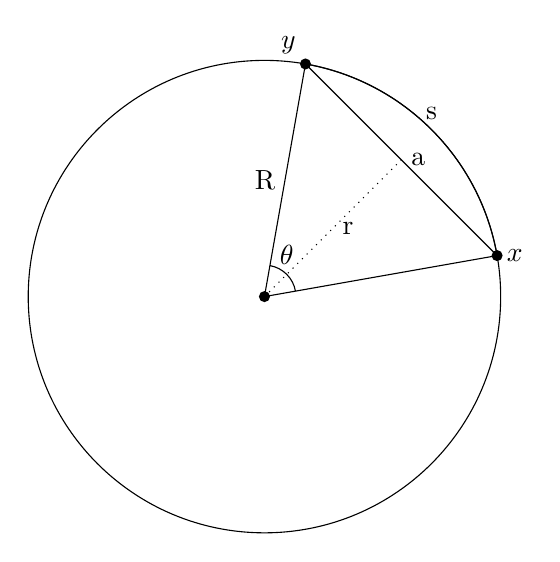
\begin{tikzpicture}
	    \draw (0,0) circle (3cm);
	    \fill (0,0) circle[radius=2pt];
	    
	    \path (0,0) ++(10:3cm) coordinate (B) node [right]{$x$};
	    \fill (B) circle[radius=2pt];
	    
	    \path (0,0) ++(80:3cm) coordinate (C) node [above left]{$y$};
	    \fill (C) circle[radius=2pt];
	    
	    \draw (0,0) -- (B) ;
	    \draw (B) arc (10:80:3cm) node[midway,above] {s};
	    \draw (B) --(C) coordinate [midway] (d) node[midway,below, right] {a};
	    \draw (C) --(0,0) node[midway,left] {R} ;
	    \draw [dotted] (0,0) -- (d) node[midway,below,right]{r};
	    \draw (10:0.4cm) arc (10:80:0.4cm) node [midway, above] {$\theta$};

	\end{tikzpicture}
\end{center}
\begin{gather}
\sin\left(\frac{\theta}{2}\right)=\frac{a/2}{R}\\
\theta = 2 \arcsin\left(\frac{a}{2R}\right)\\
a= d_e(x,y)\\
s= R\theta\\
d_i(x,y) = s = R \arcsin\left(\frac{d_e(x,y)}{2R}\right)\\
d_i(x,y) = f\circ d_e(x,y)\\
f(b) = R\arcsin\left(\frac{b}{2R}\right)
\end{gather}
It is useful to note that $\arcsin$ is only defined on the domain $[-1,1]$, and here the extrinsic metric is divided by its maximum for two points on the same sphere, $2R$, which normalizes the argument to $\arcsin$ to $[-1,1]$.

\problem{}%5
 \emph{Triangle inequality and convexity}: Let $u\to |u|$ be a function $\mathbb{R}^n \to \mathbb{R}$ satisfying
 \begin{enumerate}
 	\item $|u|\ge 0$ and $=0$ if and only if $u=0$.
 	\item $|\lambda u| =| \lambda||u|$ for all $\lambda\in \mathbb{R}$ and $u\in \mathbb{R}^n$.
 \end{enumerate}
 
 Prove that the following two statements are equivalent:
 \begin{enumerate}
 	\item $|u|$ is a norm (that is, it satisfies the triangle inequality $|u+v|\le |u| + |v|$).
 	\item For all $r>0$ the balls $B(0,r) = \{u: |u|\le r\}$ are \emph{convex} ($u,v\in B(0,r)$ and $0\le t \le 1 \Longrightarrow (1-t)u + tv \in B(0,r)$).
\end{enumerate}

\solution
\part
Suppose $|u+v|\le|u|+|v|$ and take $u,v\in B(0,r)$, $0\le\lambda\le1$, and $|u|,|v|\le r$.
\begin{align}
|\lambda u + (1-\lambda)v| &\le |\lambda u| + |(1-\lambda)v| = \lambda |u| + (1-\lambda)|v|\\
&\le \lambda r + (1-\lambda )r = r\\
|\lambda u + (1-\lambda )v| &\le r\\
& \Longrightarrow \lambda{}u + (1-\lambda{})v \in B(0,r)\\
& \rightarrow B(0,r)\text{ is convex.}
\end{align}

\part
Suppose $|\lambda u + (1-\lambda)v| \le r$ for $u,v\in B(0,r)$ and let $\lambda=0.5$.
\begin{align}
	|0.5u + (1-0.5)v| &\le r]\\
	(0.5|u+v| &\le r)\times 2\\
	 |u +v| &\le 2r \le |u| + |v|\\
	&\text{if } |u|=|v|=r
\end{align}

\end{document}
